Как было сказано в пункте 3.1: в первую очередь необходимо реализовать функции добавления клиентов в список и опрос клиентов. 

Для решения данной задачи необходимо создать класс, описывающий объект-сервер, который будет хранить список клиентов и выполнять опрос клиентов.

На данный момент нет описания к системе команд УСПД, поэтому ограничемся передачей любого тестового сообщения клиенту при помощи реализованных ранее классов-сокетов.

Так же стоит отметить что это преложение будет иметь графический интерфейс.

Прототип класса-сервера представлен ниже:

\begin{lstlisting}
class MyServer : public QObject
{
    Q_OBJECT
public:
    explicit MyServer(QObject *parent = 0);
    ~MyServer();

    void addClient(const QString &name, 
		   const QString &addr, 
		   const int &port);
    QMap<QString, ClientAddress>* getClientsList();

private:
    QMap<QString, ClientAddress> clients;
    void timerEvent(QTimerEvent* event);
};
\end{lstlisting}

В конструкторе данного класса запускается таймер, которй отсчитывает интервалы времени между опросами списка клиентов. При обнулении таймера вызывается метод timerEvent в котором и происходит опрос списка клиентов, хранящегося в QMap<QString, ClientAddress>, ClientAddress - структура данных, хранящая ip-адрес и порт назначения.

Метод addClient принимает имея, ip-адрес и порт клиента, которого необходимо добавить в список и создает новый элемент в объекте clients.

getClientsList - метод, возвращающий атрибут clients.

timerEvent - метод, который просматривает список клиентов, для каждого клиента создает свое объект типа ClienSock(описан ранее), посылает клиенту массив байт, и отключается. 

\newpage
Графический интерфейс программы представлен на рисунку \ref{server_gui:server_gui}.

\begin{figure}[ht!]
 \center{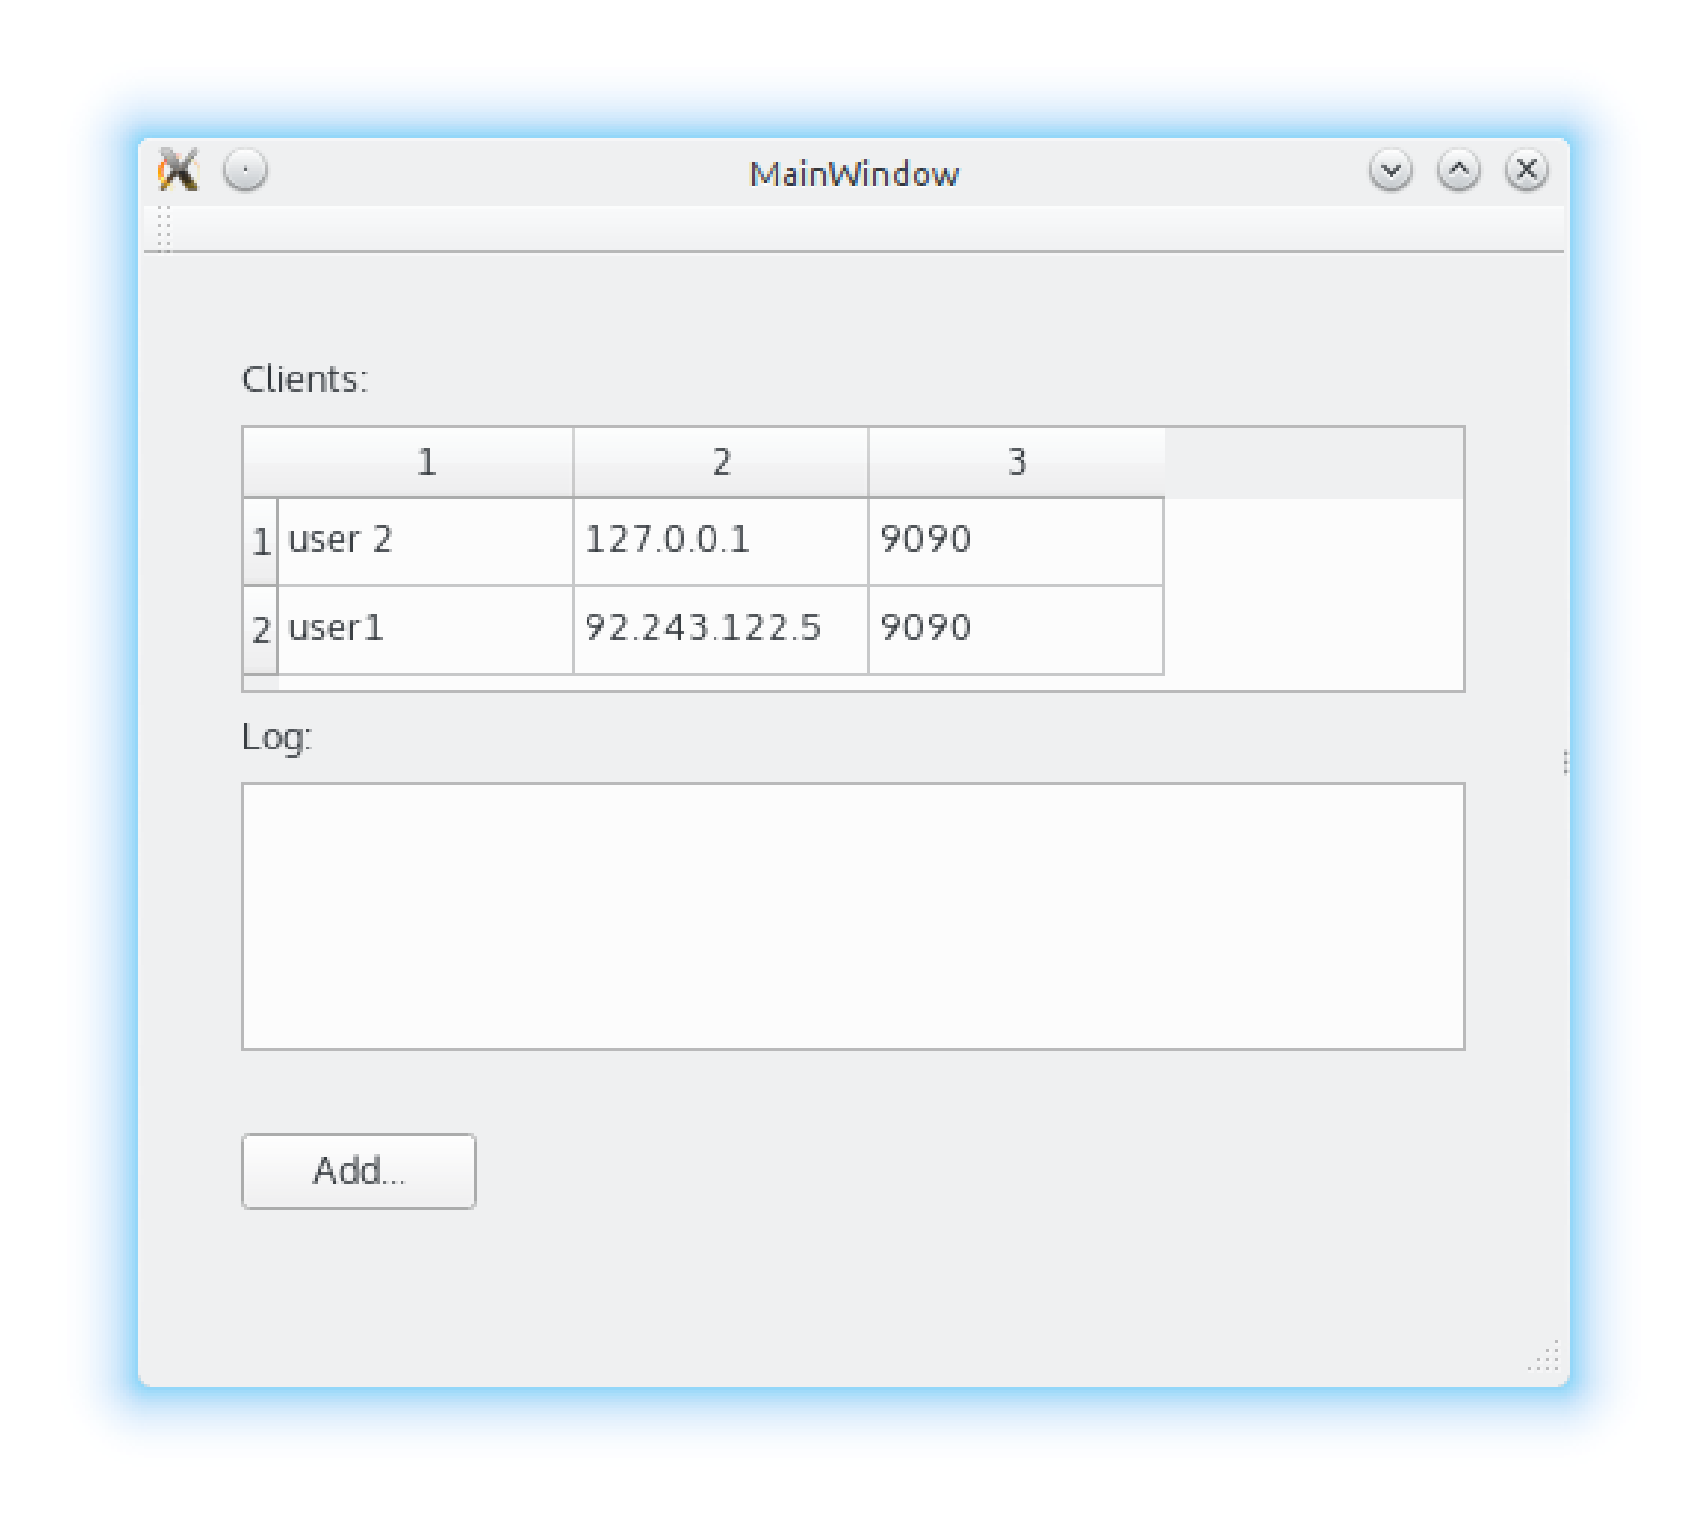
\includegraphics[width=0.7\linewidth]{server_gui}}
 \caption{интерфейс программы}
 \label{server_gui:server_gui}
\end{figure}

Реакция эмулятора УСПД на user1 представлена на рисунке \ref{client_log:client_log}.

\begin{figure}[ht!]
 \center{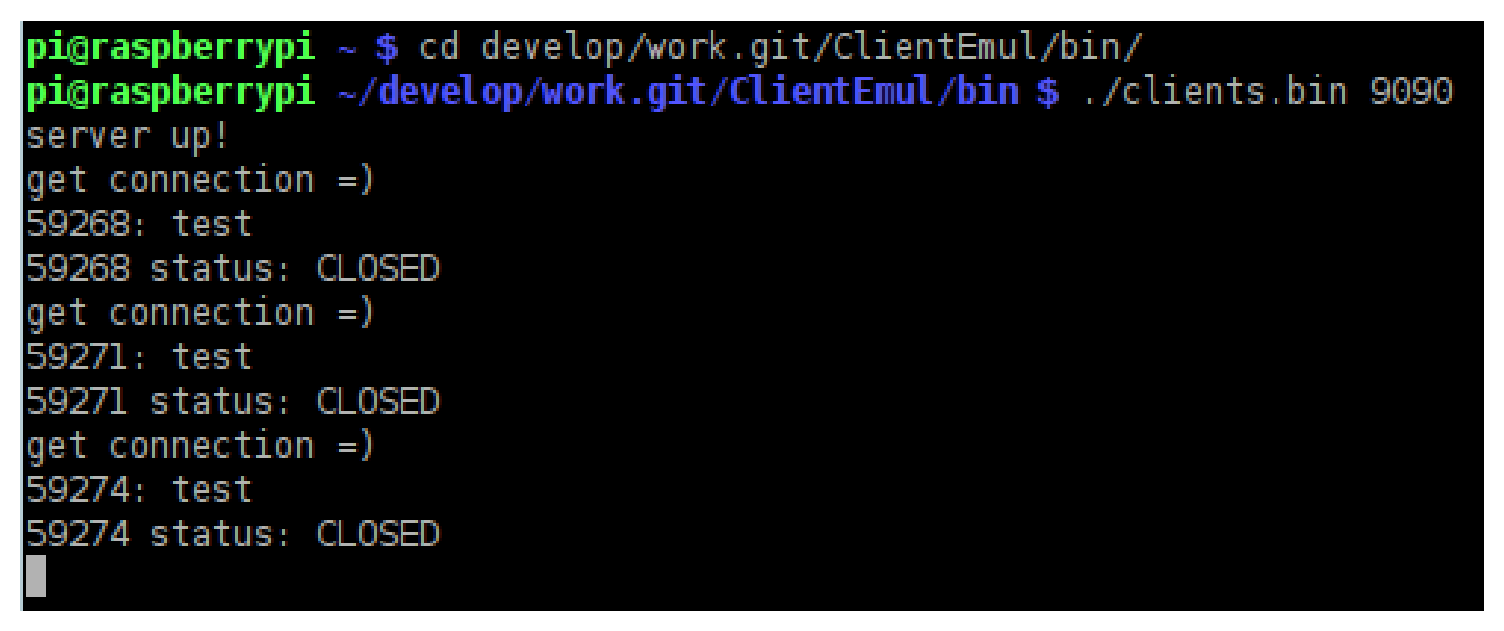
\includegraphics[width=0.7\linewidth]{client_log}}
 \caption{Работа эмулятора УСПД}
 \label{client_log:client_log}
\end{figure}



